\chapter{LPE structure}

\section{Introduction}
The techniques that are described in this document require a \txs{} model as input of which the process is in \emph{linear process equation} (LPE) \emph{form}.
Many, but not all \txs{} processes can be transformed to LPE form using the \texttt{lpe} command of \txs{}.

\section{Processes in LPE form} \label{processlpeform}

A \txs{} process
\begin{align*}
\texttt{ProcDef} \; [C_1 :: K_1, \cdots{}, C_n :: K_n] \; [p_1 :: T_1, \cdots{}, p_k :: T_k] \; b_\textit{LPE}
\end{align*}

that is identified by $P$ is said to be a in \emph{LPE form} if $b_\textit{LPE}$ follows the grammar of $\textit{LPEBody}$ below:
\begin{align*}
\textit{LPEBody} &::= \textit{ChoiceSummand} \; \;|\; \textit{ActionSummand} \\
\textit{ChoiceSummand} &::= \texttt{Choice} \; [ \;\! \textit{LPEBody}, \cdots{}, \textit{LPEBody} \; ] \\
\textit{ActionSummand} &::= \texttt{ActionPref} \; \textit{ActOffer} \; \textit{ProcInst} \\
\textit{ActOffer} &::= \texttt{ActOffer} \; \textit{ChanOffers} \;\; [ \; h_1, \cdots{}, h_z \; ] \; \textit{VExpr} \\
\textit{ChanOffers} &::= [ \;\! \textit{ChanOffer}, \cdots{}, \textit{ChanOffer} \; ] \\
\textit{ChanOffer} &::= \textit{ChanId} \;\; [\texttt{Quest} \; x_1, \cdots{}, \texttt{Quest} \; x_m] \\
\textit{ChanId} &::= C_1 \;| \cdots{} |\; C_n \;|\; \texttt{ISTEP} \;|\; \texttt{CISTEP} \\
\textit{ProcInst} &::= \texttt{ProcInst} \; P \; \; [ \; C_1, \cdots{}, C_n \; ] \; [\;\!\textit{VExpr}, \cdots{}, \textit{VExpr} \; ]
\end{align*}

Note that
\begin{itemize}
\item $b_\textit{LPE}$ should comply with traditional \txs{} requirements.
More precisely, the communication variables $\{ x_1, \cdots{}, x_m \}$ must match the signature of the \textit{ChanId} channel that occurs in the same rule; and the number of \textit{VExpr}s in the \textit{ProcInst} rule must be equal to $k$ and their sorts must match $[T_1, \cdots{}, T_k]$.
\item per summand, it must be the case that
\begin{align*}
|\; \{ h_1, \cdots{}, h_z \} \cup \{ x_1, \cdots{}, x_m \} \; | &= z + m \\
(\{ h_1, \cdots{}, h_z \} \cup \{ x_1, \cdots{}, x_m \}) \cap \{ p_1, \cdots{}, p_k \} &= \emptyset{}
\end{align*}
\end{itemize}

\section{Models in LPE form} \label{modellpeform}

In actuality, it is convenient that not just process that underlies a model is in LPE form, but that the entire model has a specific form.
Just like the specific form for processes, this form is also referred to as \emph{LPE form} because it has the same goal, namely enabling symbolic manipulation of a model.

A \txs{} model
\begin{align*}
\texttt{ModelDef} \; [I_1, \cdots{}, I_m] \; [O_1, \cdots{}, O_n] \; b_\textit{inst}
\end{align*}

is said to be in \emph{LPE form} if

\begin{itemize}
\item $I_1, \cdots{}, I_m$ are all single input channels;
\item $O_1, \cdots{}, O_n$ are all single output channels;
\item $b_\text{\textit{inst}}$ has the form
\begin{align*}
\texttt{ProcInst} \; P \; [D_1, \cdots{}, D_{m+n}] \; [v_I(p_1), \cdots{}, v_I(p_k)]
\end{align*}

such that
\begin{align*}
\{ I_1, \cdots{}, I_m \}, \{ O_1, \cdots{}, O_n \} \subseteq \{ D_1, \cdots{}, D_{m+n} \}
\end{align*}

and
\begin{align*}
\{ I_1, \cdots{}, I_m \} \cap \{ O_1, \cdots{}, O_n \} = \emptyset{}
\end{align*}

\item the \txs{} process that is identified by $P$ is
\begin{align*}
\texttt{ProcDef} \; [C_1 :: K_1, \cdots{}, C_{m+n} :: K_{m+n}] \; [p_1 :: T_1, \cdots{}, p_k :: T_k] \; b_\textit{LPE}
\end{align*}
such that
\begin{align*}
\text{type}(C_i) = \text{type}(D_i) = K_i &\text{ for all } i \in [1, \cdots{}, m+n] \\
\text{type}(v_I(p_i)) = T_i &\text{ for all } i \in [1, \cdots{}, k]
\end{align*}

\item the \txs{} process that is identified by $P$ is in LPE form conform \ref{processlpeform}.
\end{itemize}

\section{Model linearization}

A model can be converted to LPE form in a way that is reversible.

Let the input LPE model be $M$ and the underlying LPE be $P$.
Let the form of the $i$th summand of LPE $P$ be defined by 
\begin{align*}
s_i = \Gamma_i(1) \; \texttt{|} \; &\cdots{} \; \texttt{|} \; \Gamma_i(m_i) \; H_i \; [[g_i]] \text{ \texttt{>->} } P(v_i(p_1), \cdots{}, v_i(p_k)) \\
\Gamma_i(j) &= c_i(j) \; \texttt{?} \; x_{i,j}(1) \; \cdots{} \; \texttt{?} \; x_{i,j}(n_{i,j}) \\
H_i &= \texttt{?} \; h_{i}(1) \; \cdots{} \; \texttt{?} \; h_{i}(z_{i})
\end{align*}

where

\begin{itemize}
\item $\Gamma_i(1) \; \texttt{|} \; \cdots{} \; \texttt{|} \; \Gamma_i(m_i)$ are the \textit{ChanOffers} of summand $s_i$, of which there are $m_i \geq 0$;
\item $c_i(j)$ is the channel name of the $j$th \textit{ChanOffer} of summand $s_i$;
\item $x_{i,j}(e)$ is the $e$th communication variable of the $j$th \textit{ChanOffer} of summand $s_i$;
\item $n_{i,j}$ is the number of communication variables of the $j$th \textit{ChanOffer} of summand $s_i$;
\item $H_i$ are the hidden variables of summand $s_i$, of which there are $z_i$;
\item $h_i(e)$ is the $e$th hidden variable of summand $s_i$;
\item $g_i$ is the guard of summand $s_i$ (the only free variables in this expression must be parameters of $P$, communication variables of summand $s_i$, or hidden variables of summand $s_i$);
\item $p_1, \cdots{}, p_k$ are the parameters of $P$, of which there are $k \geq 0$;
\item $v_i(p)$ is an expression that defines the new value of parameter $p$ of $P$ after the application of summand $s_i$ (the only free variables in this expression must be LPE parameters, communication variables of summand $s_i$, or hidden variables of summand $s_i$).
\end{itemize}

Define a \emph{channel signature} as a pair $(C, S)$ where $C$ is an ordered list of channels and $S$ is an ordered list of sorts, and define a function $\tau$ that yields the channel signature of a summand $s_i$:
\begin{align*}
\tau(s_i) = (&[ c_i(1), \cdots{}, c_i(m_i)], \\
&[\flsortof{c_i(1)}, \cdots{}, \flsortof{c_i(m_i)}, \sortof{h_i(1)}, \cdots{}, \sortof{h_i(z_i)}])
\end{align*}

where $\text{flsort} = \text{flatten} \circ{} \text{sort}$ and
\begin{align*}
\text{flatten}(k_1 \; \texttt{\#\#} \cdots{} \texttt{\#\#} \; k_q) = [k_1, \cdots{}, k_q]
\end{align*}

for some $q > 0$.

Define an injective function $\theta(T)$ that maps channel signature
\begin{align*}
T = (C, [s_1, \cdots{}, s_{m_i+z_i}])
\end{align*}

to a fresh, uniquely named channel with sort $s_1 \; \texttt{\#\#} \cdots{} \texttt{\#\#} \; s_{m_i+z_i}$.

Given these definitions, do the following:

\begin{enumerate}
\item For each summand $s_i$, compute $\tau(s_i)$.
Add the results to a set $\Sigma$.

\item Compute $\Omega = \{ (\sigma, \theta(\sigma)) \;|\; \sigma \in \Sigma \}$.

\item For each summand $s_i$, look up a pair $(a, b) \in \Omega$ so that $a = \tau(s_i)$.
There is only one such pair.
Change the action offer of $s_i$ to
\begin{align*}
a \; {\Gamma_i(1)}' \; &\cdots{} \; {\Gamma_i(m_i)}' \; H_i \\
{\Gamma_i(j)}' &= \texttt{?} \; x_{i,j}(1) \; \cdots{} \; \texttt{?} \; x_{i,j}(n_{i,j})
\end{align*}

\item Compute $\Theta = \{ b \;|\; (a, b) \in \Omega \}$.

\item Update $M$ and $P$ so that $P$ has access to the channels in $\Theta$.
Be consistent in the order of channel parameter values when instantiating $P$!
\end{enumerate}

Given $\Omega$, how to reverse the procedure above should be obvious.

\section{Data structure}

The implementation stores a \txs{} model that is in LPE form in a dedicated data structure before any of the techniques that are described in this document are applied.
A visual representation of this data structure can be found in Figure~\ref{lpedatastructure:fig}.

\begin{figure}[!ht]
\begin{center}
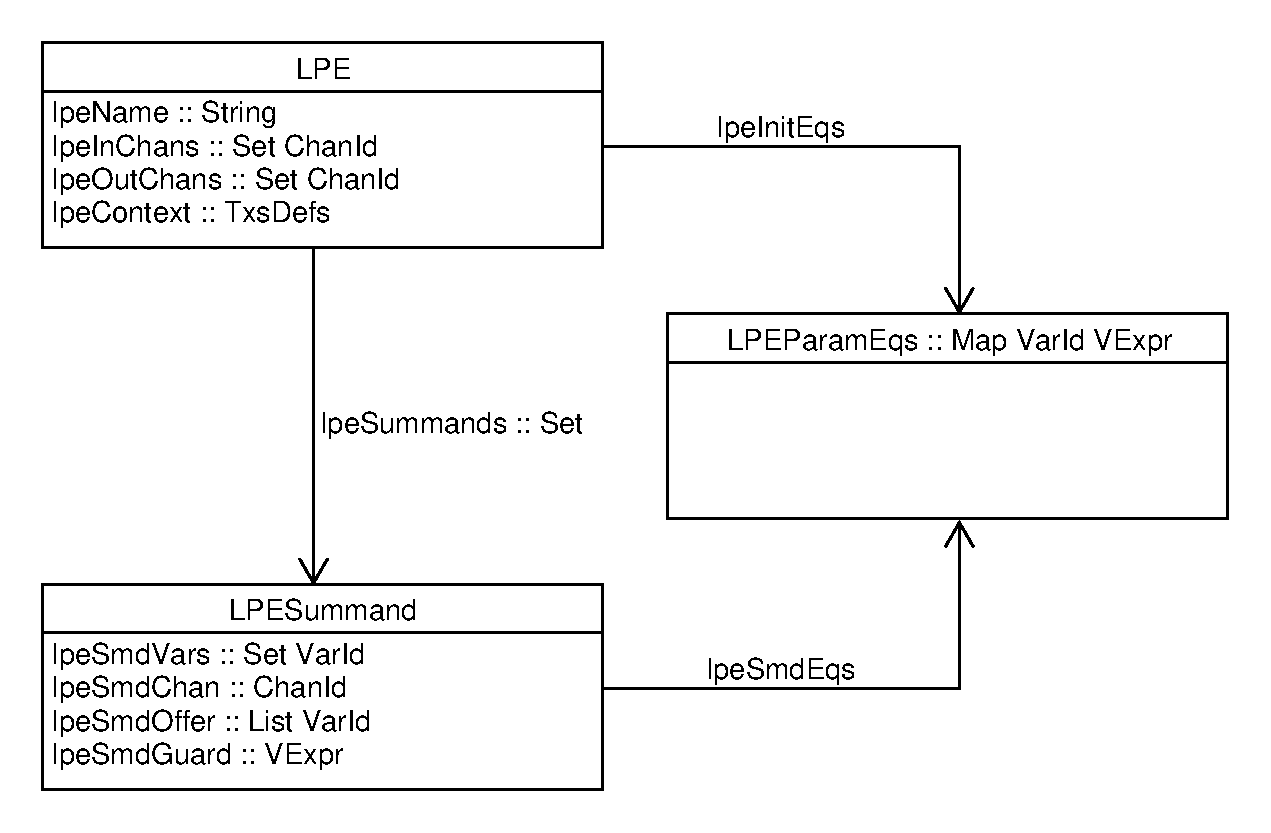
\includegraphics[width=0.7\linewidth]{images/lpe-types}
\caption{LPE data structure.}
\label{lpedatastructure:fig}
\end{center}
\end{figure}

The main data type is \texttt{LPE}.
This type primarily contains information about the \txs{} process in LPE form:
\begin{itemize}
\item The name of the LPE process is \texttt{lpeName};
\item The tree structure of \textit{ActionSummand}s that was allowed by the grammar of LPEs (see \ref{processlpeform}) has been flattened in the new data structure, resulting in a set of \texttt{LPESummand} objects; and
\item The sorts of the data parameters of the LPE process are contained in \texttt{lpeInitEqs} as well as how each data parameter is initialized.
\end{itemize}

Because the LPE process is always instantiated with the same channels in the same order, the \texttt{LPE} type only has to track which channels are input channels (\texttt{lpeInChans}) and which channels are output channels (\texttt{lpeOutChans}).
Note, however, that these are single channel identifiers that may have been freshly generated from multi-channel summands or from summands with hidden variables (see \ref{modellinearization}).
The \texttt{lpeChanMap} defines how channels in the LPE data structure are converted back to the original channels.

The \texttt{LPE} type also stores some circumstantial information in \texttt{lpeContext}.
This is a library of \txs{} type and function definitions that has been copied directly from the original \txs{} model specification.
It is used to validate instances of the \texttt{LPE} type, to generate default values of a specific sort, and more.

Finally, the \texttt{LPESummand} type only contains information about a specific summand: \texttt{lpeSmdChan} is the channel over which it communicates; \texttt{lpeSmdOffers} are the communication variables (including variables that originally were hidden variables); and the \texttt{lpeSmdEqs} map defines which expressions are used to assign new values to the parameters of the LPE after the application of the summand.

\section{Model linearization} \label{modellinearization}

The previous section briefly touched on how models are converted to LPE form.
This section goes into more detail on this subject.

Converting a model to LPE form requires the creation of a mapping from multi-channels to fresh, single channels.
For example,

TODO

Every scenario where summands have hidden variables ($h_1, \cdots{}, h_z$) also requires a dedicated channel definition.

TODO

\section{Summand elements} \label{summandelements}

To formally reference the elements of $s_i$ -- the $i$th summand of LPE $P$ -- the following definition is used:
\begin{align*}
s_i = C_i \; \texttt{?} \; x_i(1) \; \cdots{} \; \texttt{?} \; x_i(m_i) \; [[g_i]] \text{ \texttt{>->} } P(v_i(p_1), \cdots{}, v_i(p_k))
\end{align*}

where

\begin{itemize}
\item $C_i$ is the name of the channel over which summand $s_i$ communicates (if there is no such channel, \istep{} or \cistep{} is used);
\item $m_i \geq 0$ is the number of variables that summand $s_i$ uses locally, such as communication variables and hidden variables;
\item $x_i(j)$ is the $j$th variable that summand $s_i$ uses locally (communication variables first, followed by hidden variables);
\item $g_i$ is the guard of summand $s_i$ (the only free variables in this expression must be parameters of $P$, communication variables of summand $s_i$, or hidden variables of summand $s_i$);
\item $p_1, \cdots{}, p_k$ are the parameters of $P$, of which there are $k \geq 0$;
\item $v_i(p)$ is an expression that defines the new value of parameter $p$ of $P$ after the application of summand $s_i$ (the only free variables in this expression must be LPE parameters, communication variables of summand $s_i$, or hidden variables of summand $s_i$).
\end{itemize}

